\chapter{Applikation}
Dieses Kapitel beschreibt die begleitende Anwendung und deren Bedienoberfläche sowie die zentralen Funktionen für die Auswertung der Tachographendaten. Zudem werden geplante Erweiterungen skizziert, um den künftigen Funktionsumfang einzuordnen.

\section{Technische Eigenschaften der App}
Die Anwendung ist als clientseitige, mobile Applikation konzipiert, die die Kommunikation mit dem ESP32 übernimmt und die ausgelesenen Daten lokal verarbeitet. Im Fokus stehen Offlinefähigkeit, kurze Antwortzeiten und eine klare Trennung von Datenübertragung, Parsing und Darstellung. Die Architektur ist modular aufgebaut, sodass Kommunikationslogik, Datenmodell und UI weitgehend entkoppelt sind. Zustandsänderungen wie Verbindungsstatus, Downloadfortschritt und Parse-Ergebnis werden zentral erfasst und in der Oberfläche konsistent dargestellt.

Die Anwendung fungiert als Client für das ESP32-basierte Auslesegerät. Die Übertragung der Tachographendateien im \code{.ddd}-Format erfolgt über \gls{ble}. Nach dem Download werden die Dateien lokal geparst und in eine strukturierte Datenrepräsentation überführt, die die spätere Auswertung und Visualisierung ermöglicht.
Die strukturierte Repräsentation bildet die Grundlage für Filter, Zeitansichten, Statistiken und Kartenansichten, sodass die Ergebnisse in unterschiedlichen Perspektiven konsistent dargestellt werden können.

Im aktuellen Prototyp liegt der Schwerpunkt auf der lokalen Verarbeitung ohne serverseitige Persistenz. Eine Anbindung an Nutzerkonten und Datenbanken ist als Erweiterung vorgesehen und wird im Abschnitt zu den geplanten Erweiterungen aufgegriffen.

\section{Funktionen der App}
Die folgenden Screenshots veranschaulichen den aktuellen Stand der Applikation und ordnen die wichtigsten Funktionen den Ansichten zu.
\begin{figure}[H]
  \centering
  \begin{minipage}[b]{0.31\linewidth}
    \centering
    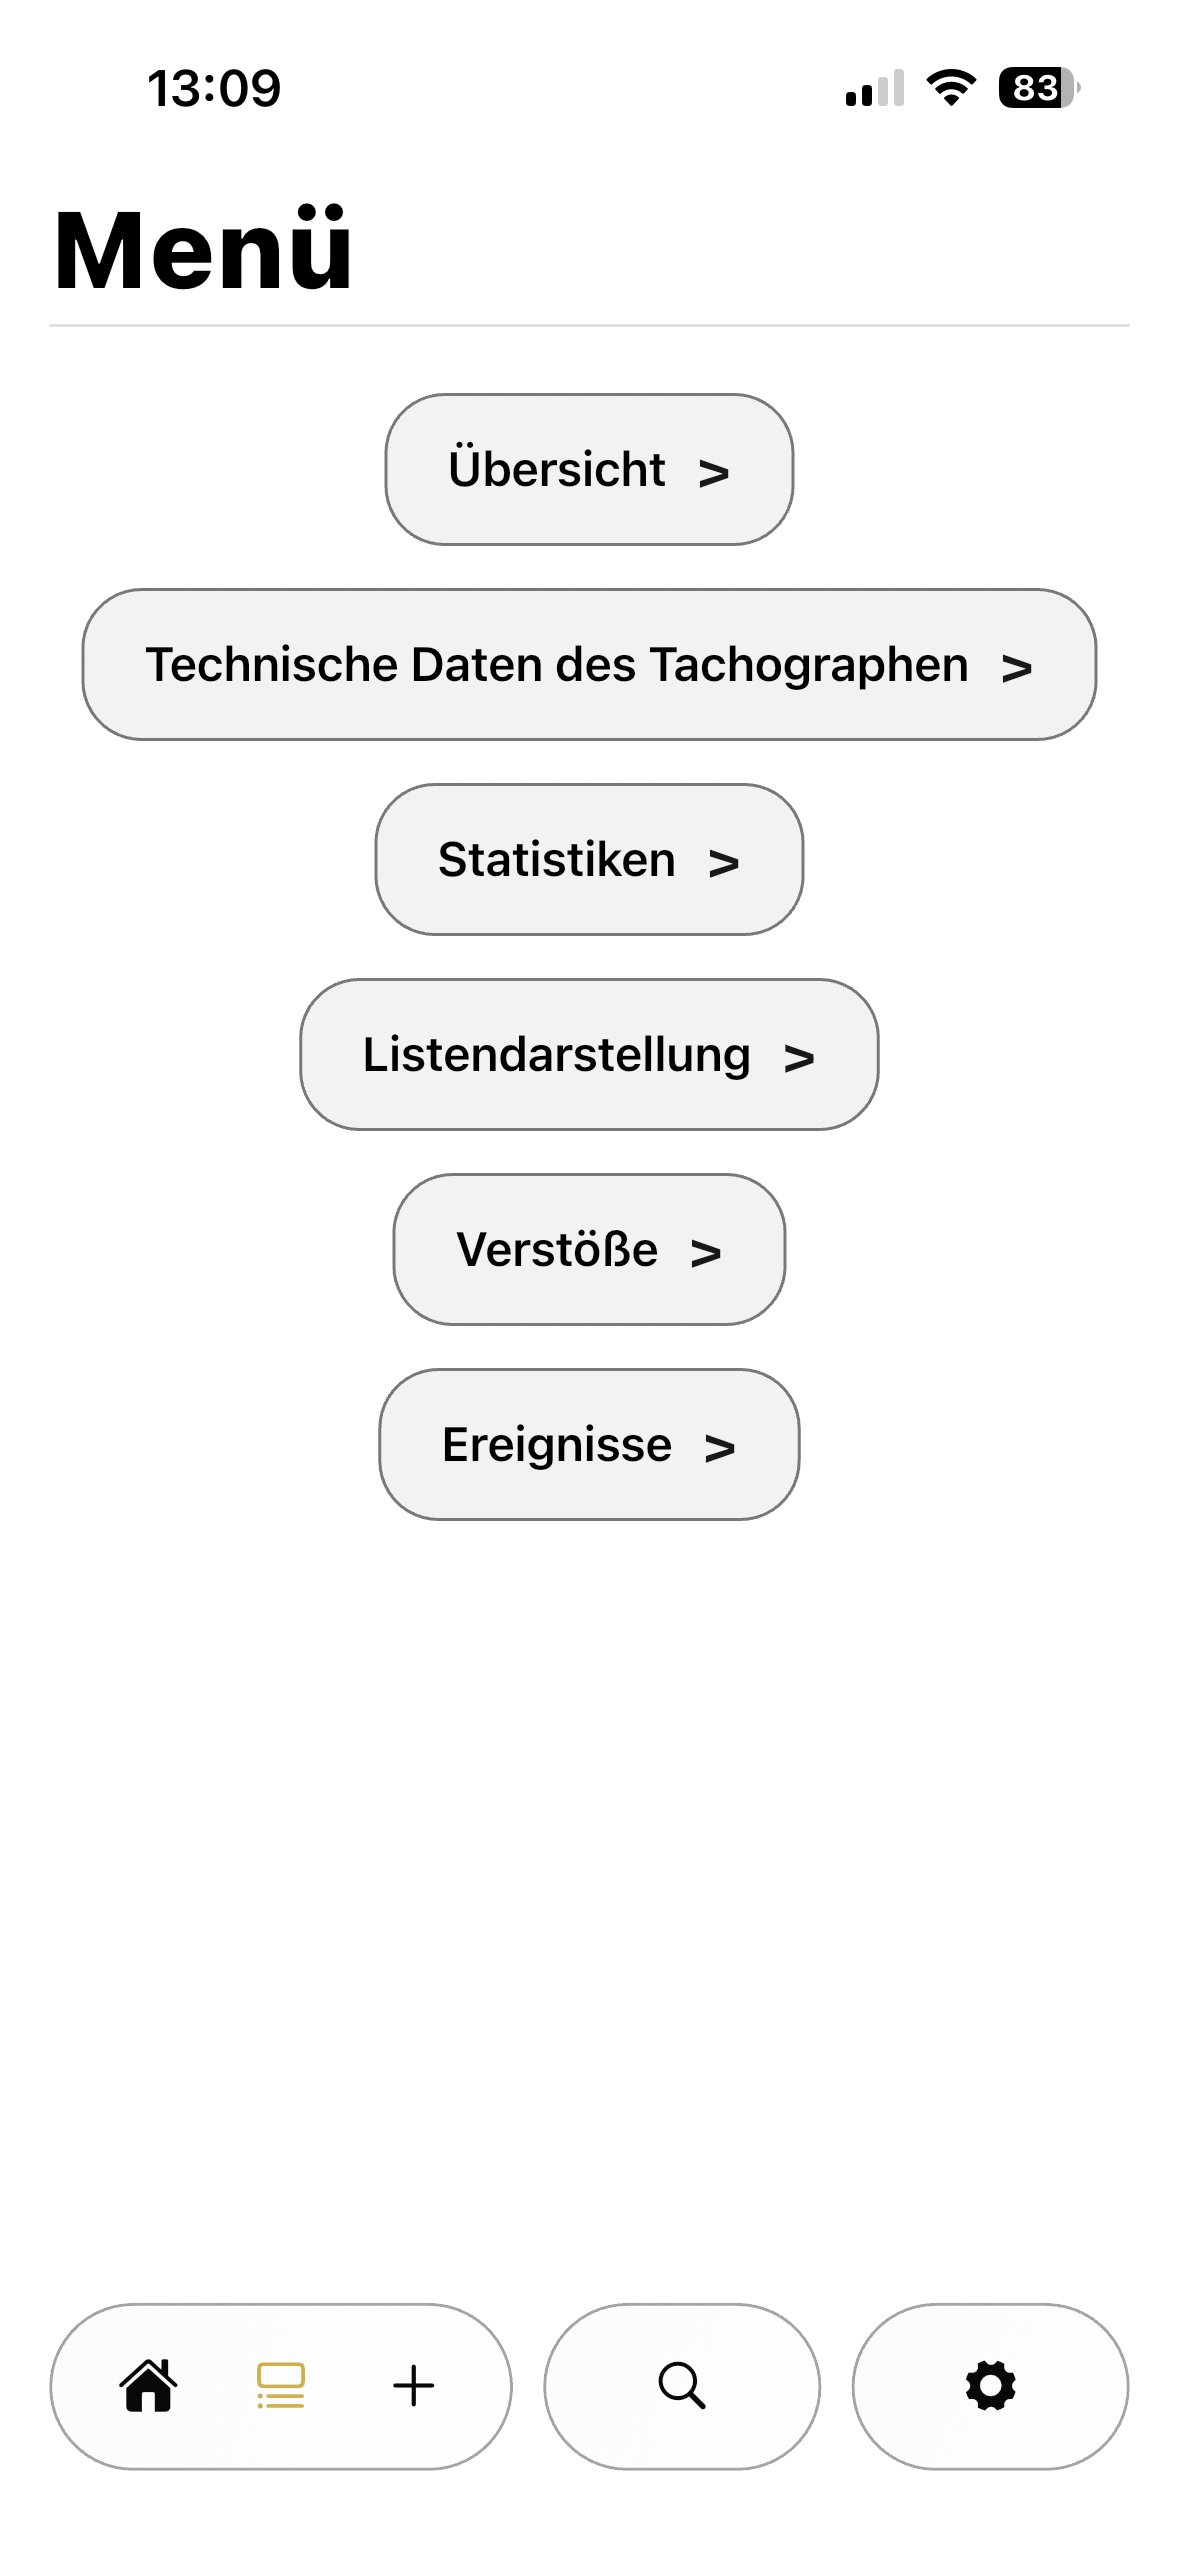
\includegraphics[width=\linewidth]{bilder/app1.png}
  \end{minipage}
  \hfill
  \begin{minipage}[b]{0.31\linewidth}
    \centering
    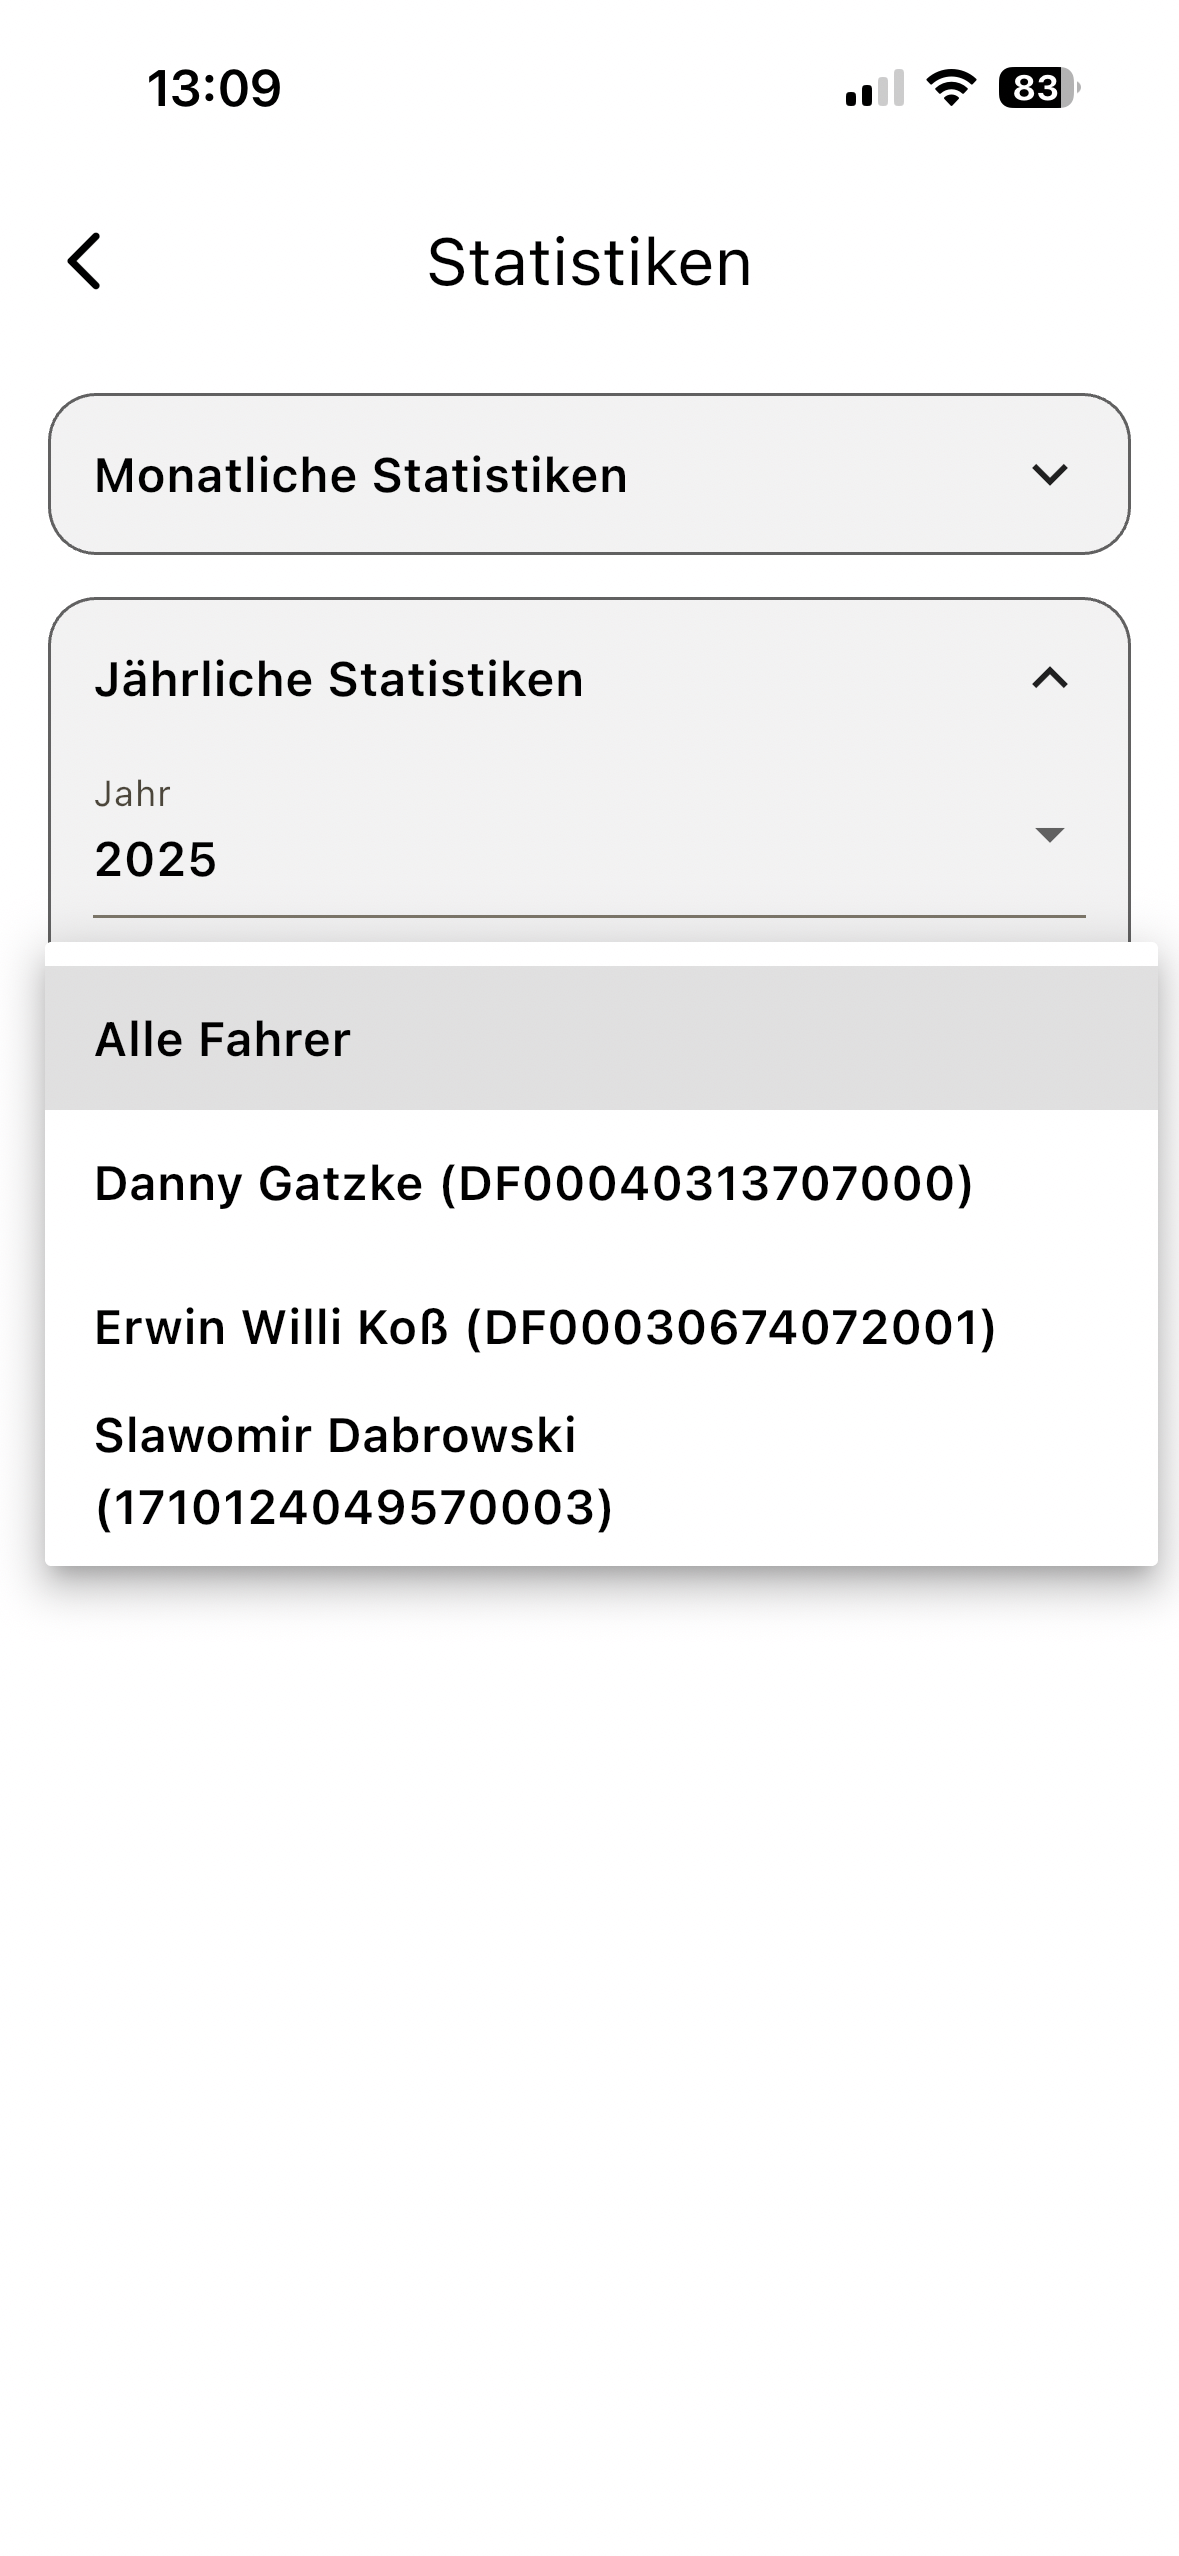
\includegraphics[width=\linewidth]{bilder/app2.png}
  \end{minipage}
  \hfill
  \begin{minipage}[b]{0.31\linewidth}
    \centering
    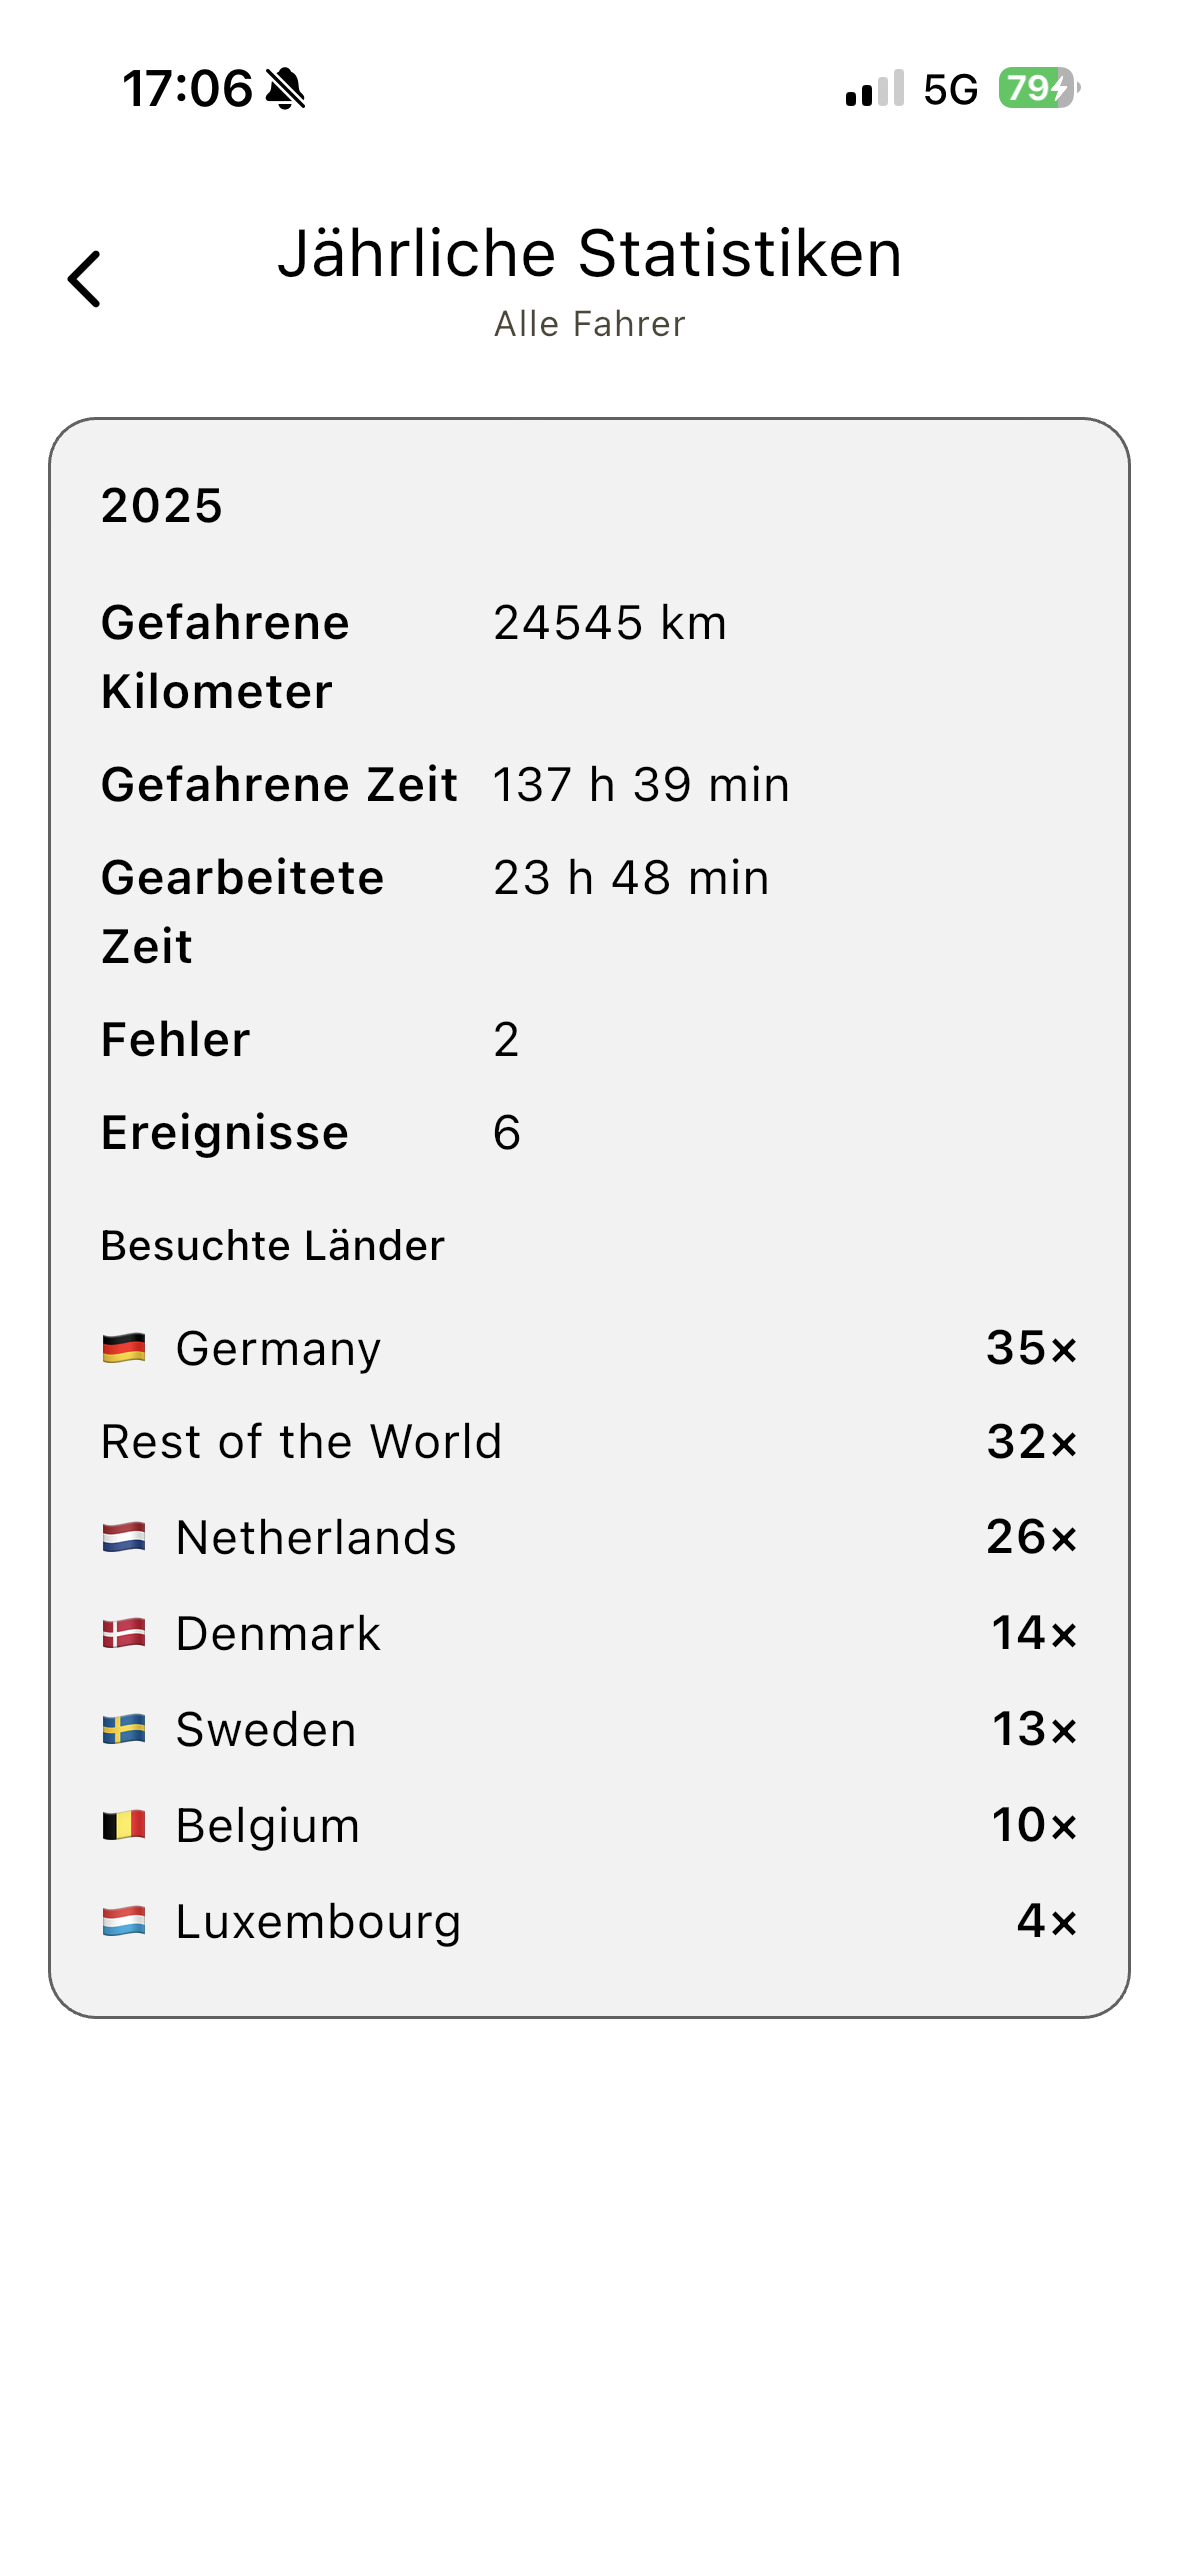
\includegraphics[width=\linewidth]{bilder/app9.png}
  \end{minipage}
  \caption{Hauptmenu der Applikation und Einblick ins Statistikenauswahlmenu.}
  \label{fig:app-ui-grid1}
\end{figure}
Der Zugriff auf die App erfolgt über einen Demo-User. Eine Navigationsleiste am unteren Bildschirmrand strukturiert die Hauptbereiche, sodass die wichtigsten Funktionen auf mobilen Endgeräten schnell erreichbar sind. Im Statistikbereich können Auswertungen für alle oder einzelne Fahrer angezeigt werden, beispielsweise besuchte Länder in einem definierten Zeitraum sowie Fahr- und Arbeitsstunden. Die Oberfläche bietet einen Dark- und einen Light-Mode, zudem lässt sich die Akzentfarbe anpassen.

\begin{figure}[H]
  \centering
  \begin{minipage}[b]{0.31\linewidth}
    \centering
    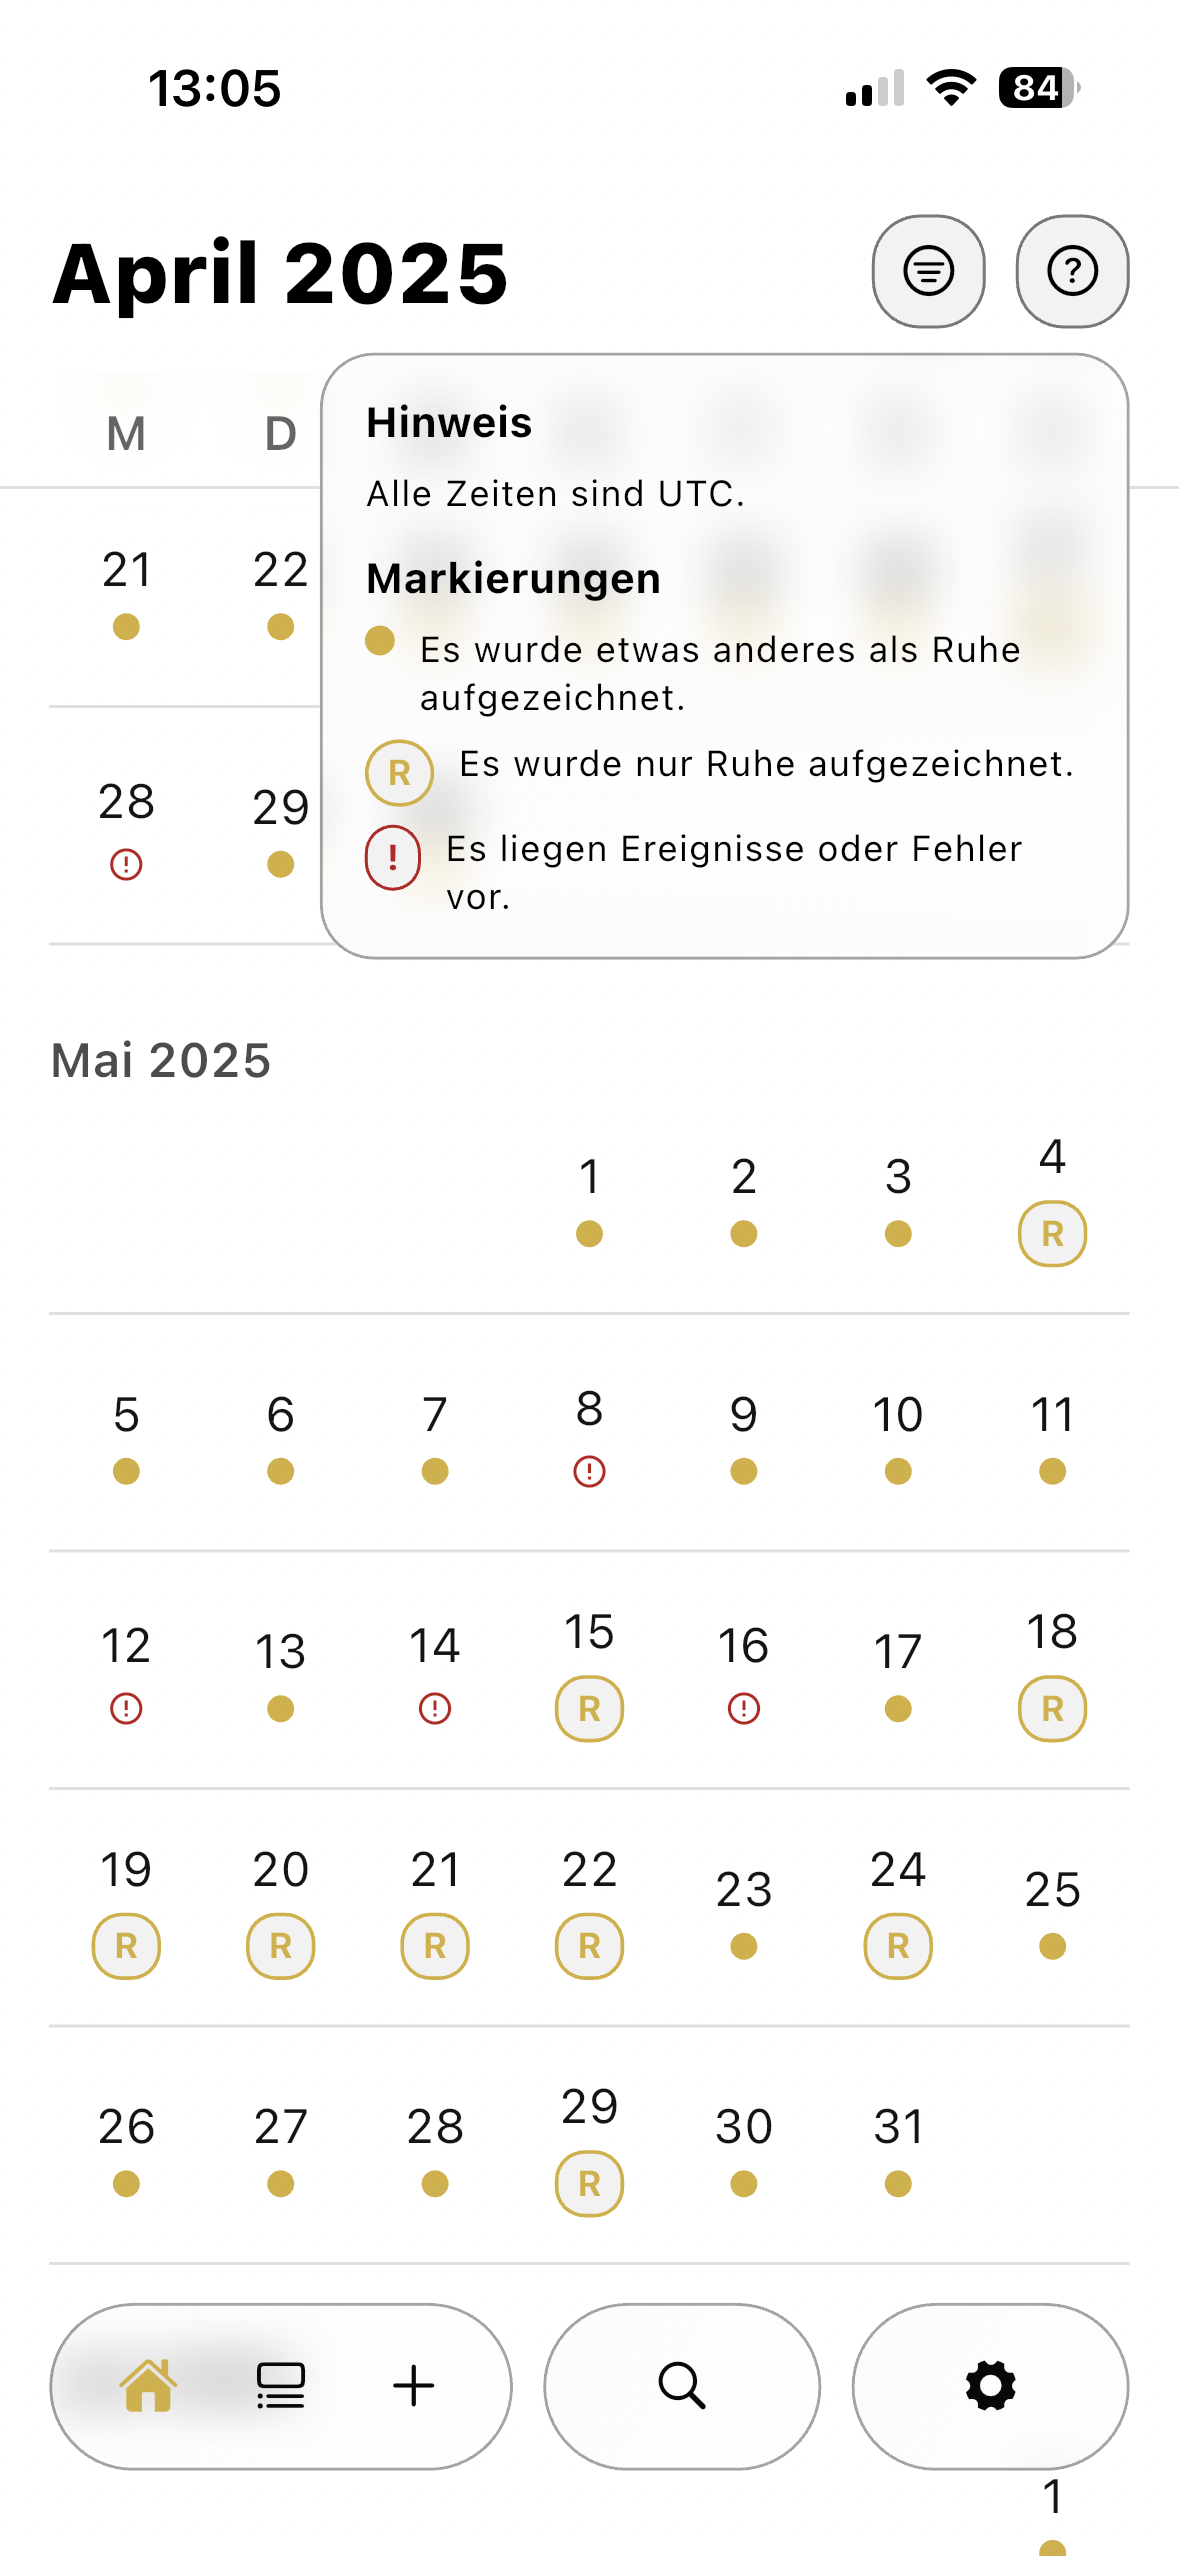
\includegraphics[width=\linewidth]{bilder/app3.png}
  \end{minipage}
  \hfill
  \begin{minipage}[b]{0.31\linewidth}
    \centering
    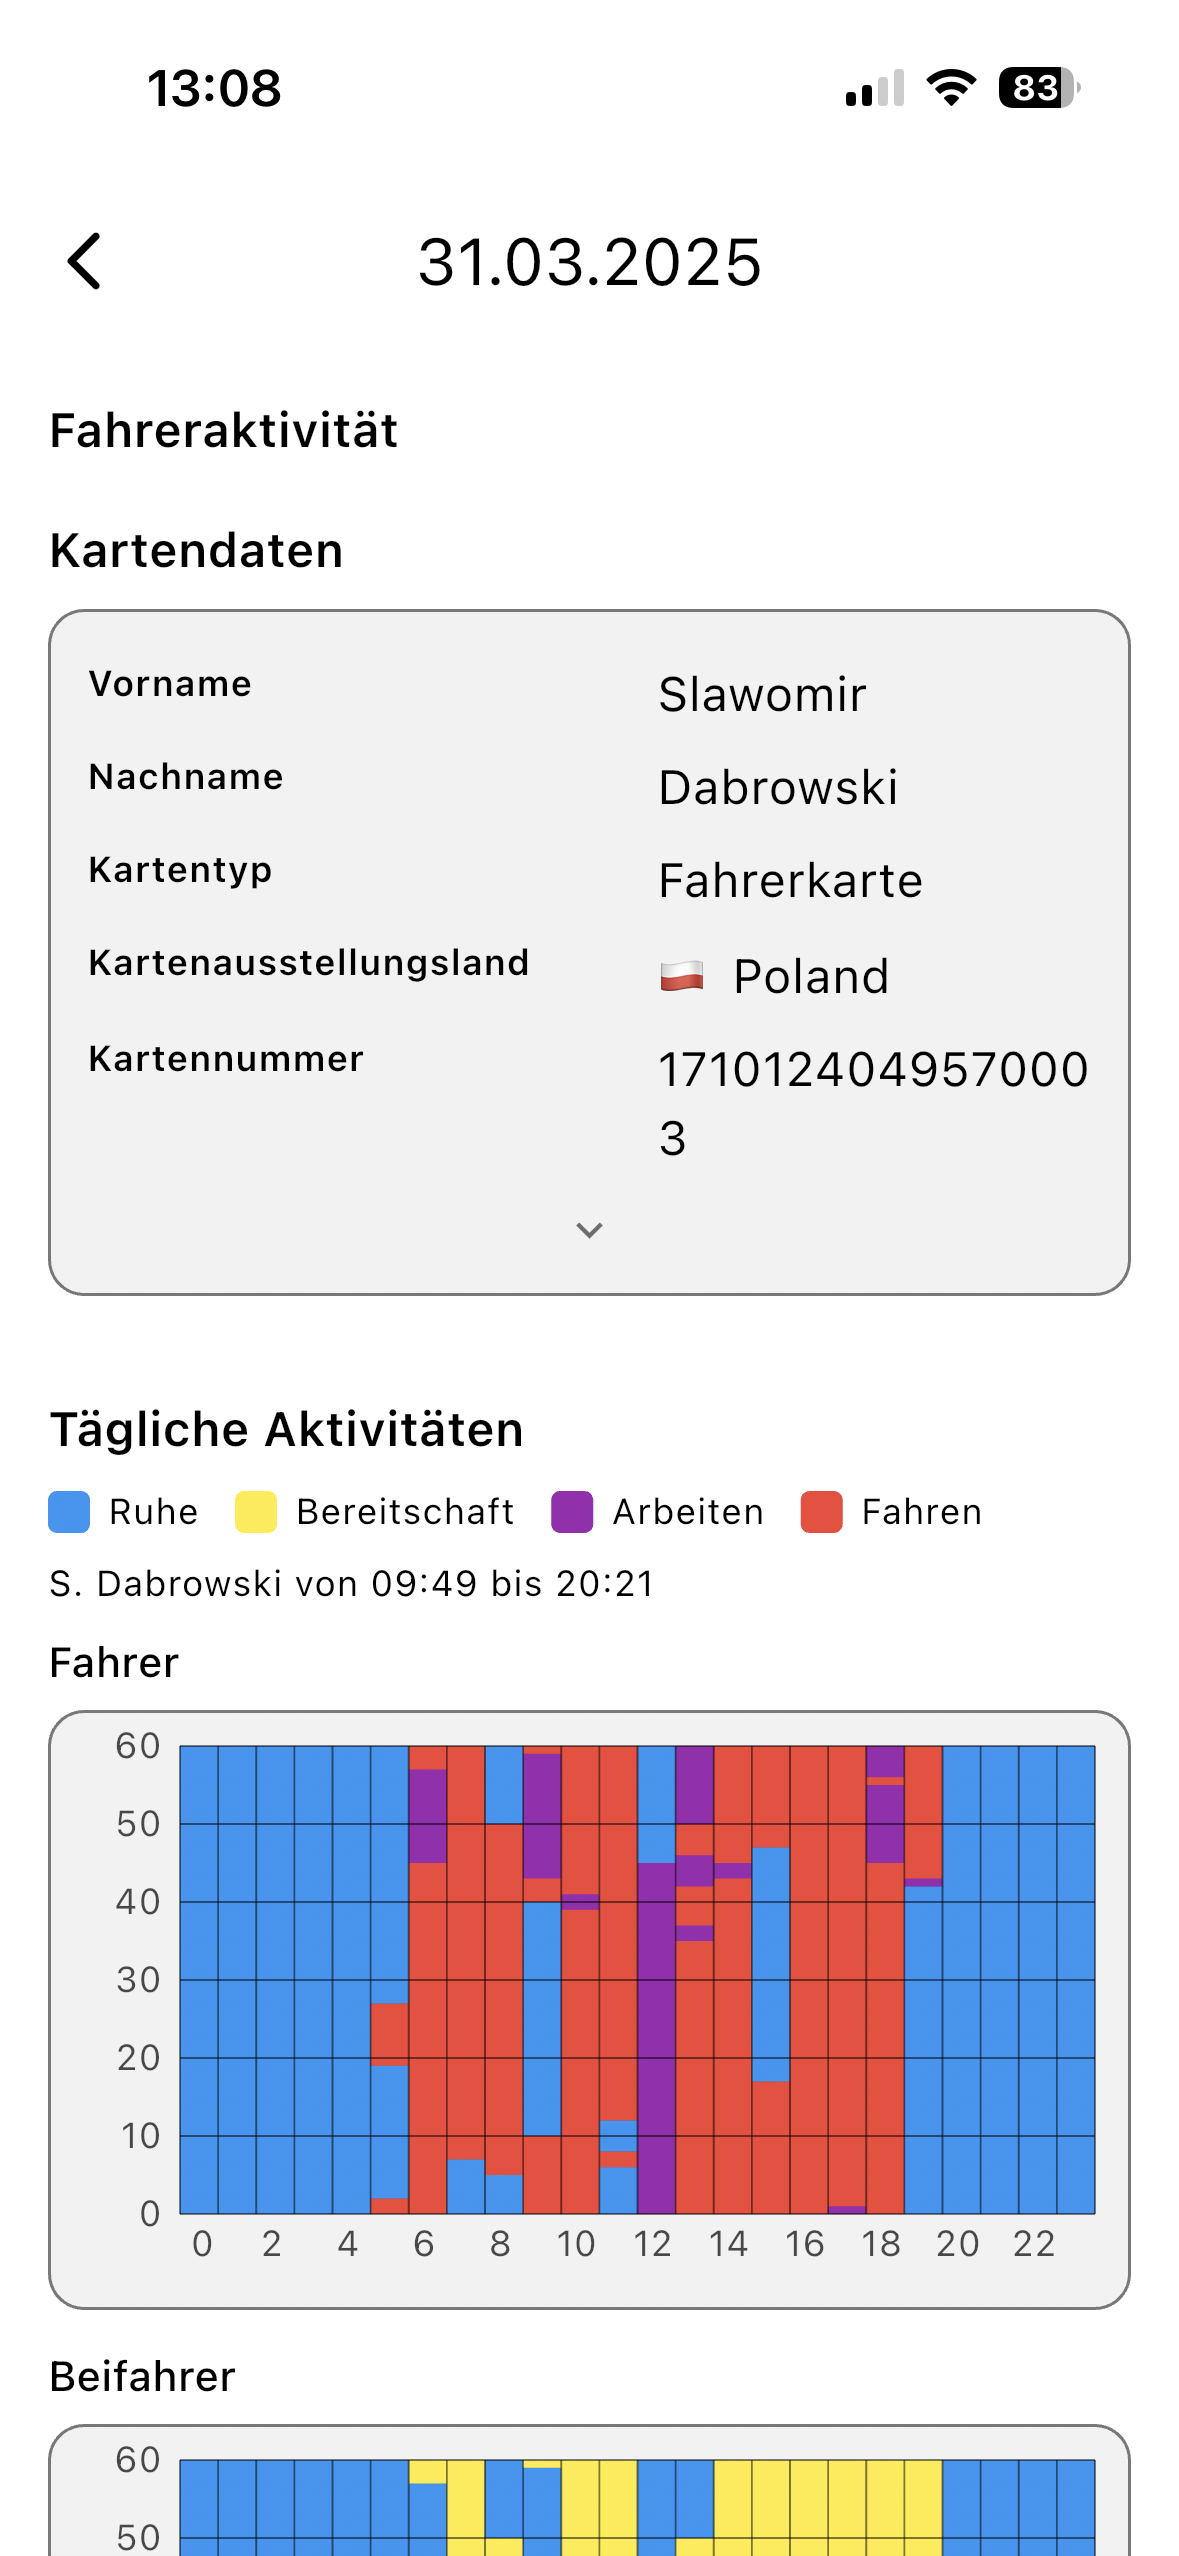
\includegraphics[width=\linewidth]{bilder/app4.png}
  \end{minipage}
  \hfill
  \begin{minipage}[b]{0.31\linewidth}
    \centering
    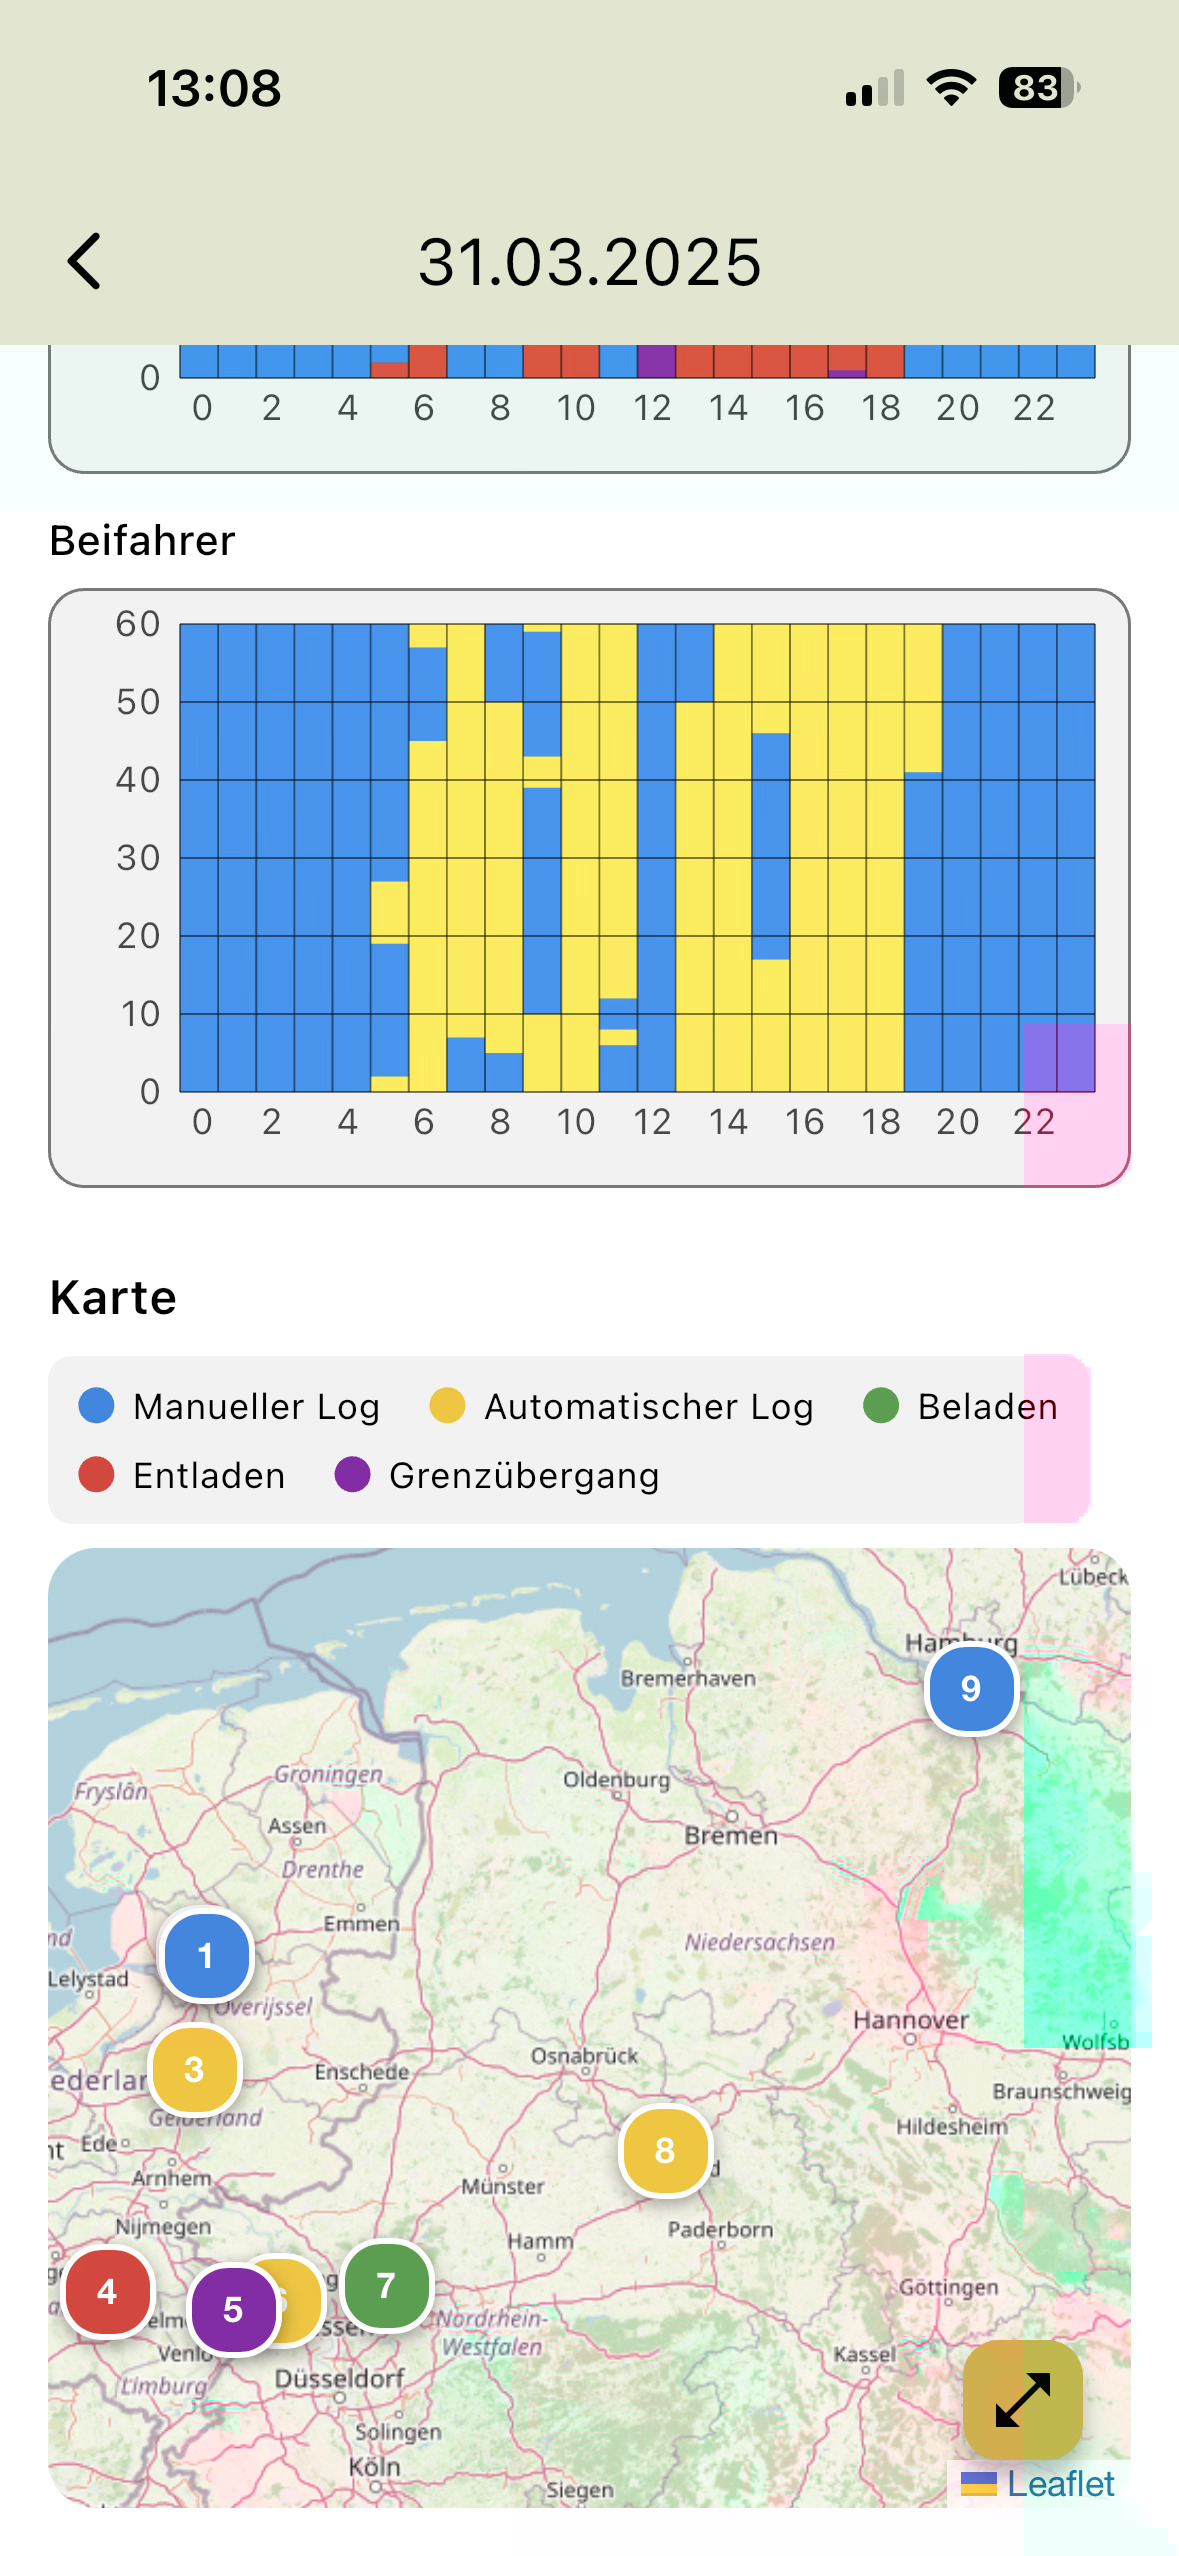
\includegraphics[width=\linewidth]{bilder/app5.png}
  \end{minipage}
  \caption{Kalenderansicht der App und Detailansicht eines einzelnen Tages.}
  \label{fig:app-ui-grid2}
\end{figure}
Die Kalenderansicht ist die Standarddarstellung; alternativ steht eine Listenansicht zur Verfügung. Filter ermöglichen es, bestimmte Marker gezielt auszublenden. In der Detailansicht werden die täglichen Aktivitäten zusammengeführt und in Ruhe, Bereitschaft, Arbeiten und Fahren gegliedert. \gls{gnss-gloss}-Positionen sind als farbige Indikatoren auf der Karte sichtbar, um den Ursprung der Messungen nachvollziehbar zu machen. Zudem werden manuelle Logeinträge, etwa beim Stecken oder Entfernen der Karte, sowie automatische Logs, Belade- und Entladevorgänge und Grenzübergänge angezeigt; Grenzübergangsmarkierungen sind anklickbar und zeigen das verlassene und das betretene Land. Die Ansicht kann außerdem auf Ereignisse und Fehler eingeschränkt werden.

\begin{figure}[H]
  \centering
  \begin{minipage}[b]{0.31\linewidth}
    \centering
    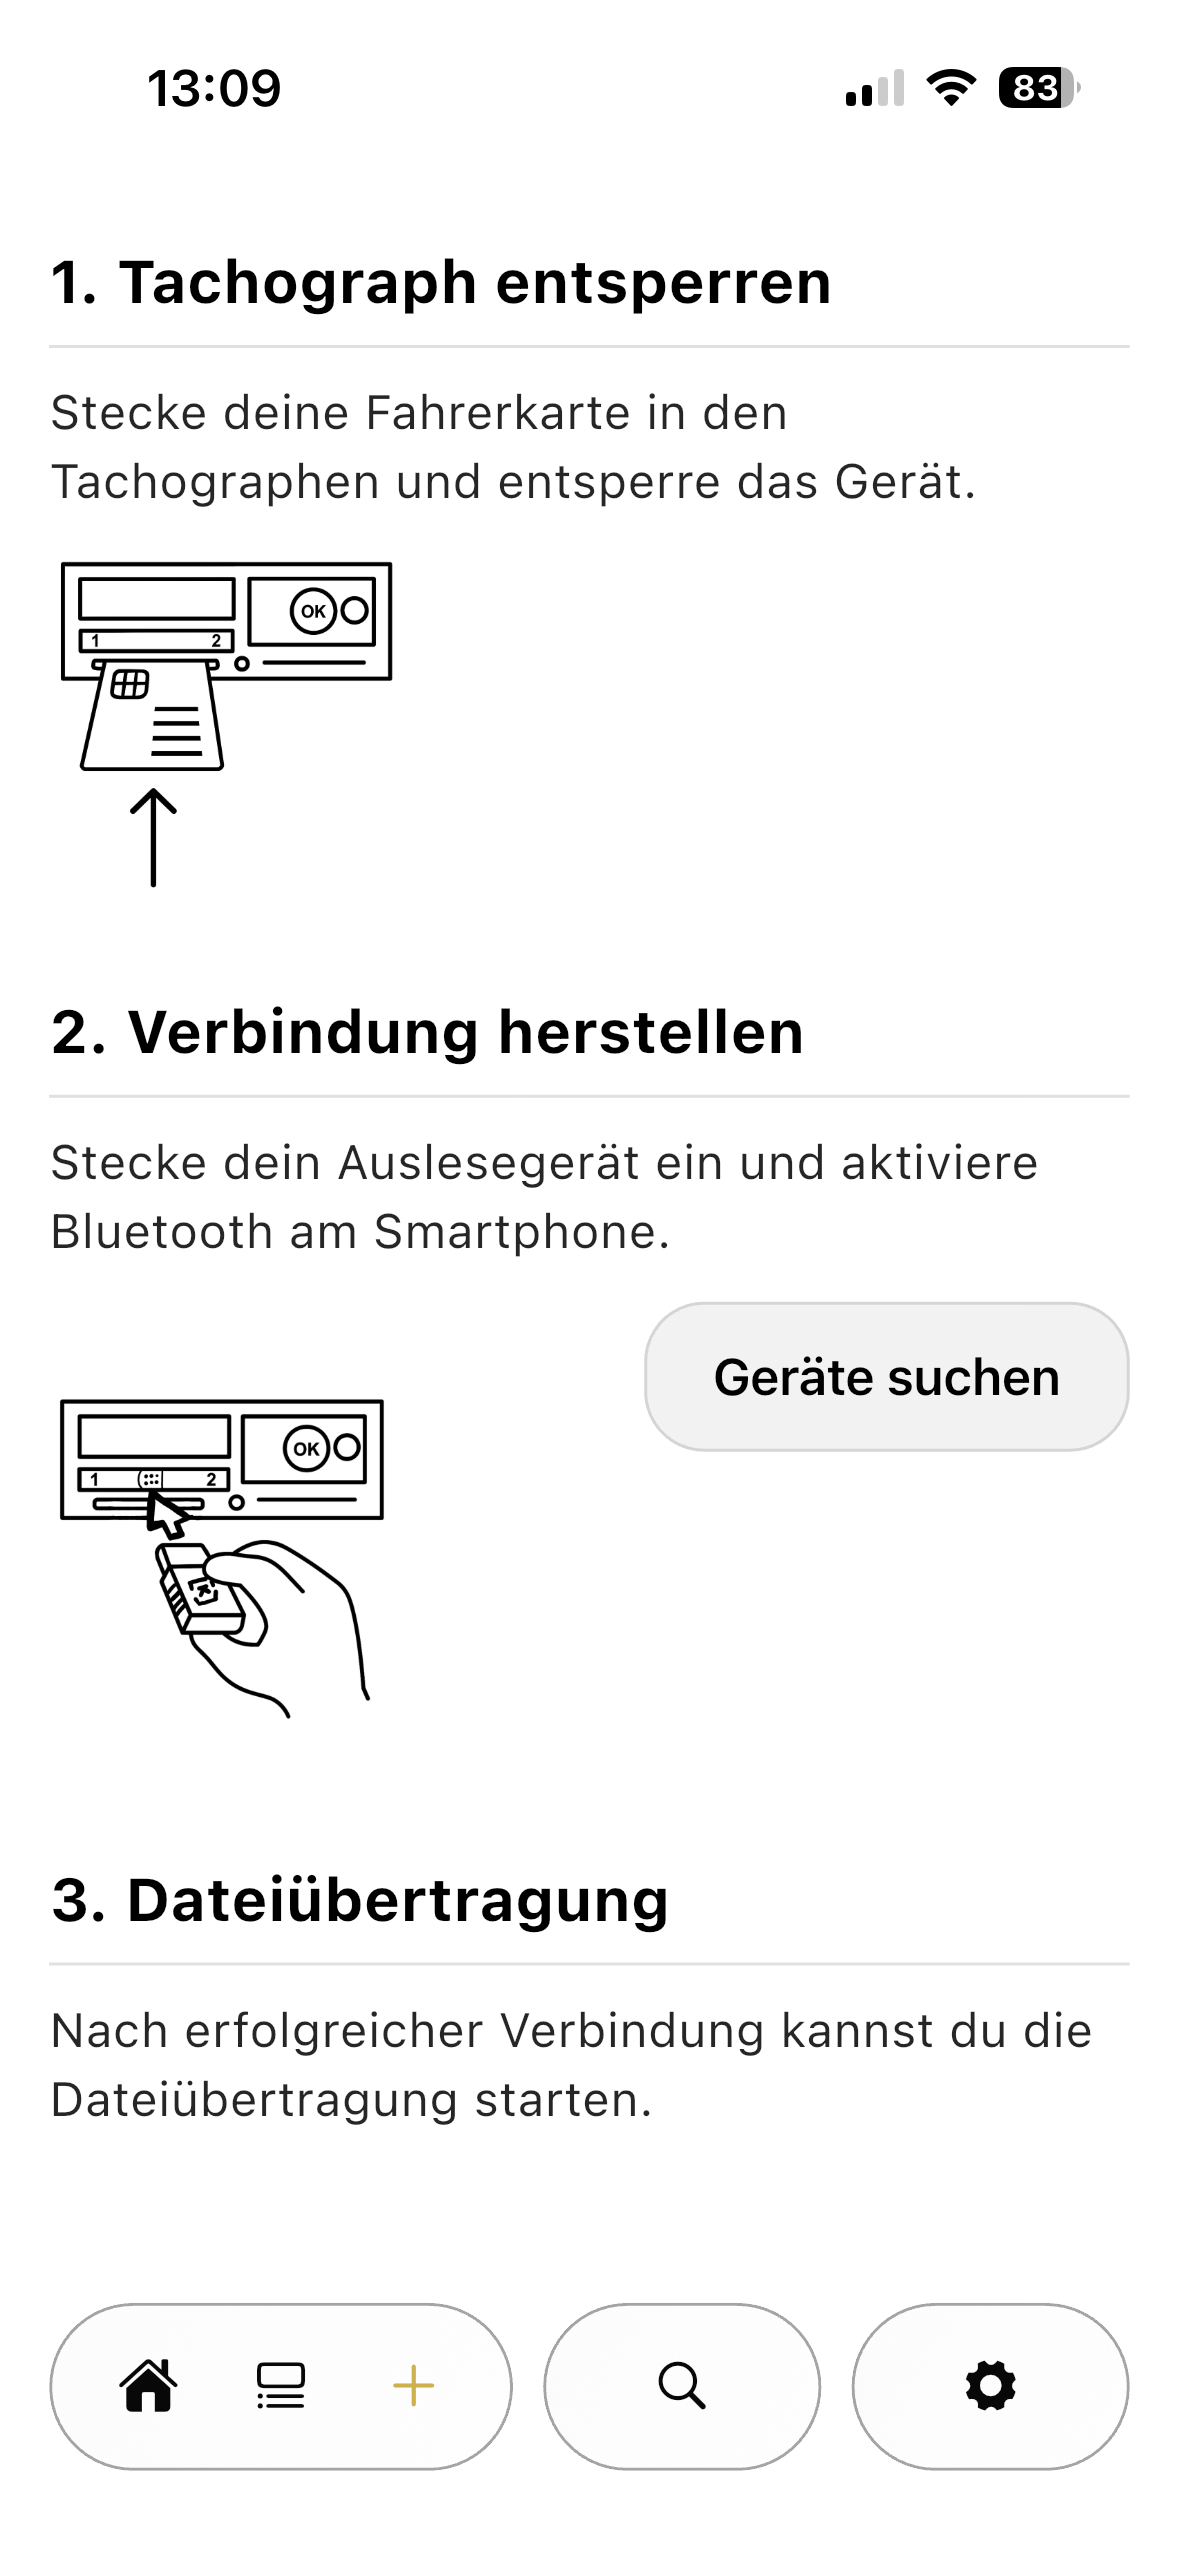
\includegraphics[width=\linewidth]{bilder/app6.png}
  \end{minipage}
  \hfill
  \begin{minipage}[b]{0.31\linewidth}
    \centering
    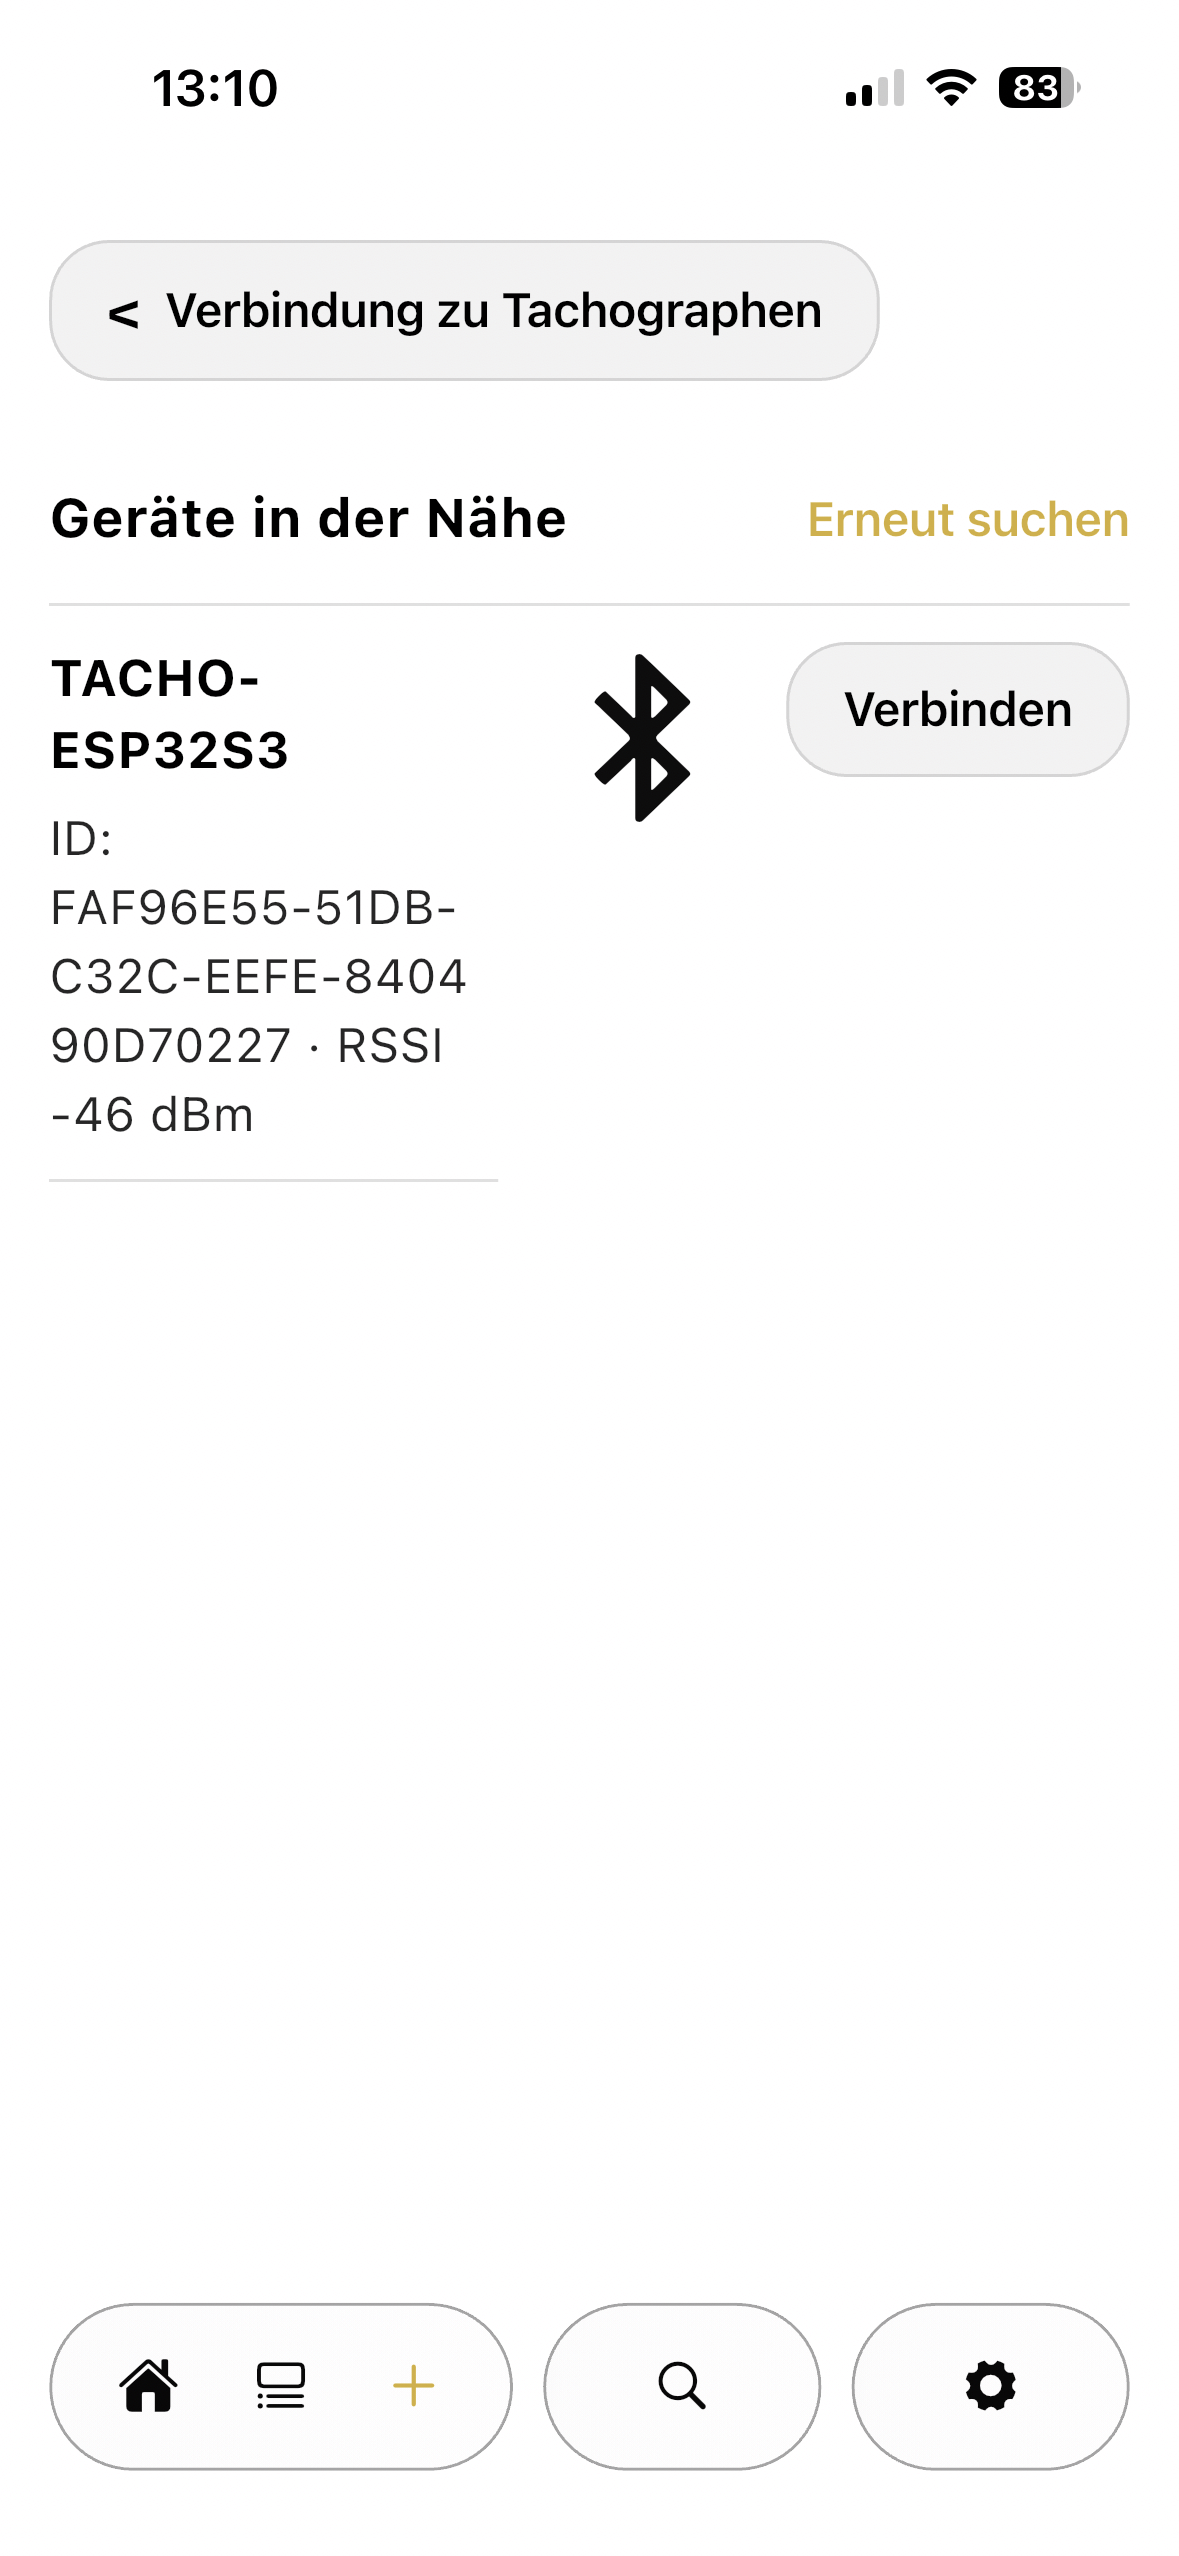
\includegraphics[width=\linewidth]{bilder/app7.png}
  \end{minipage}
  \hfill
  \begin{minipage}[b]{0.31\linewidth}
    \centering
    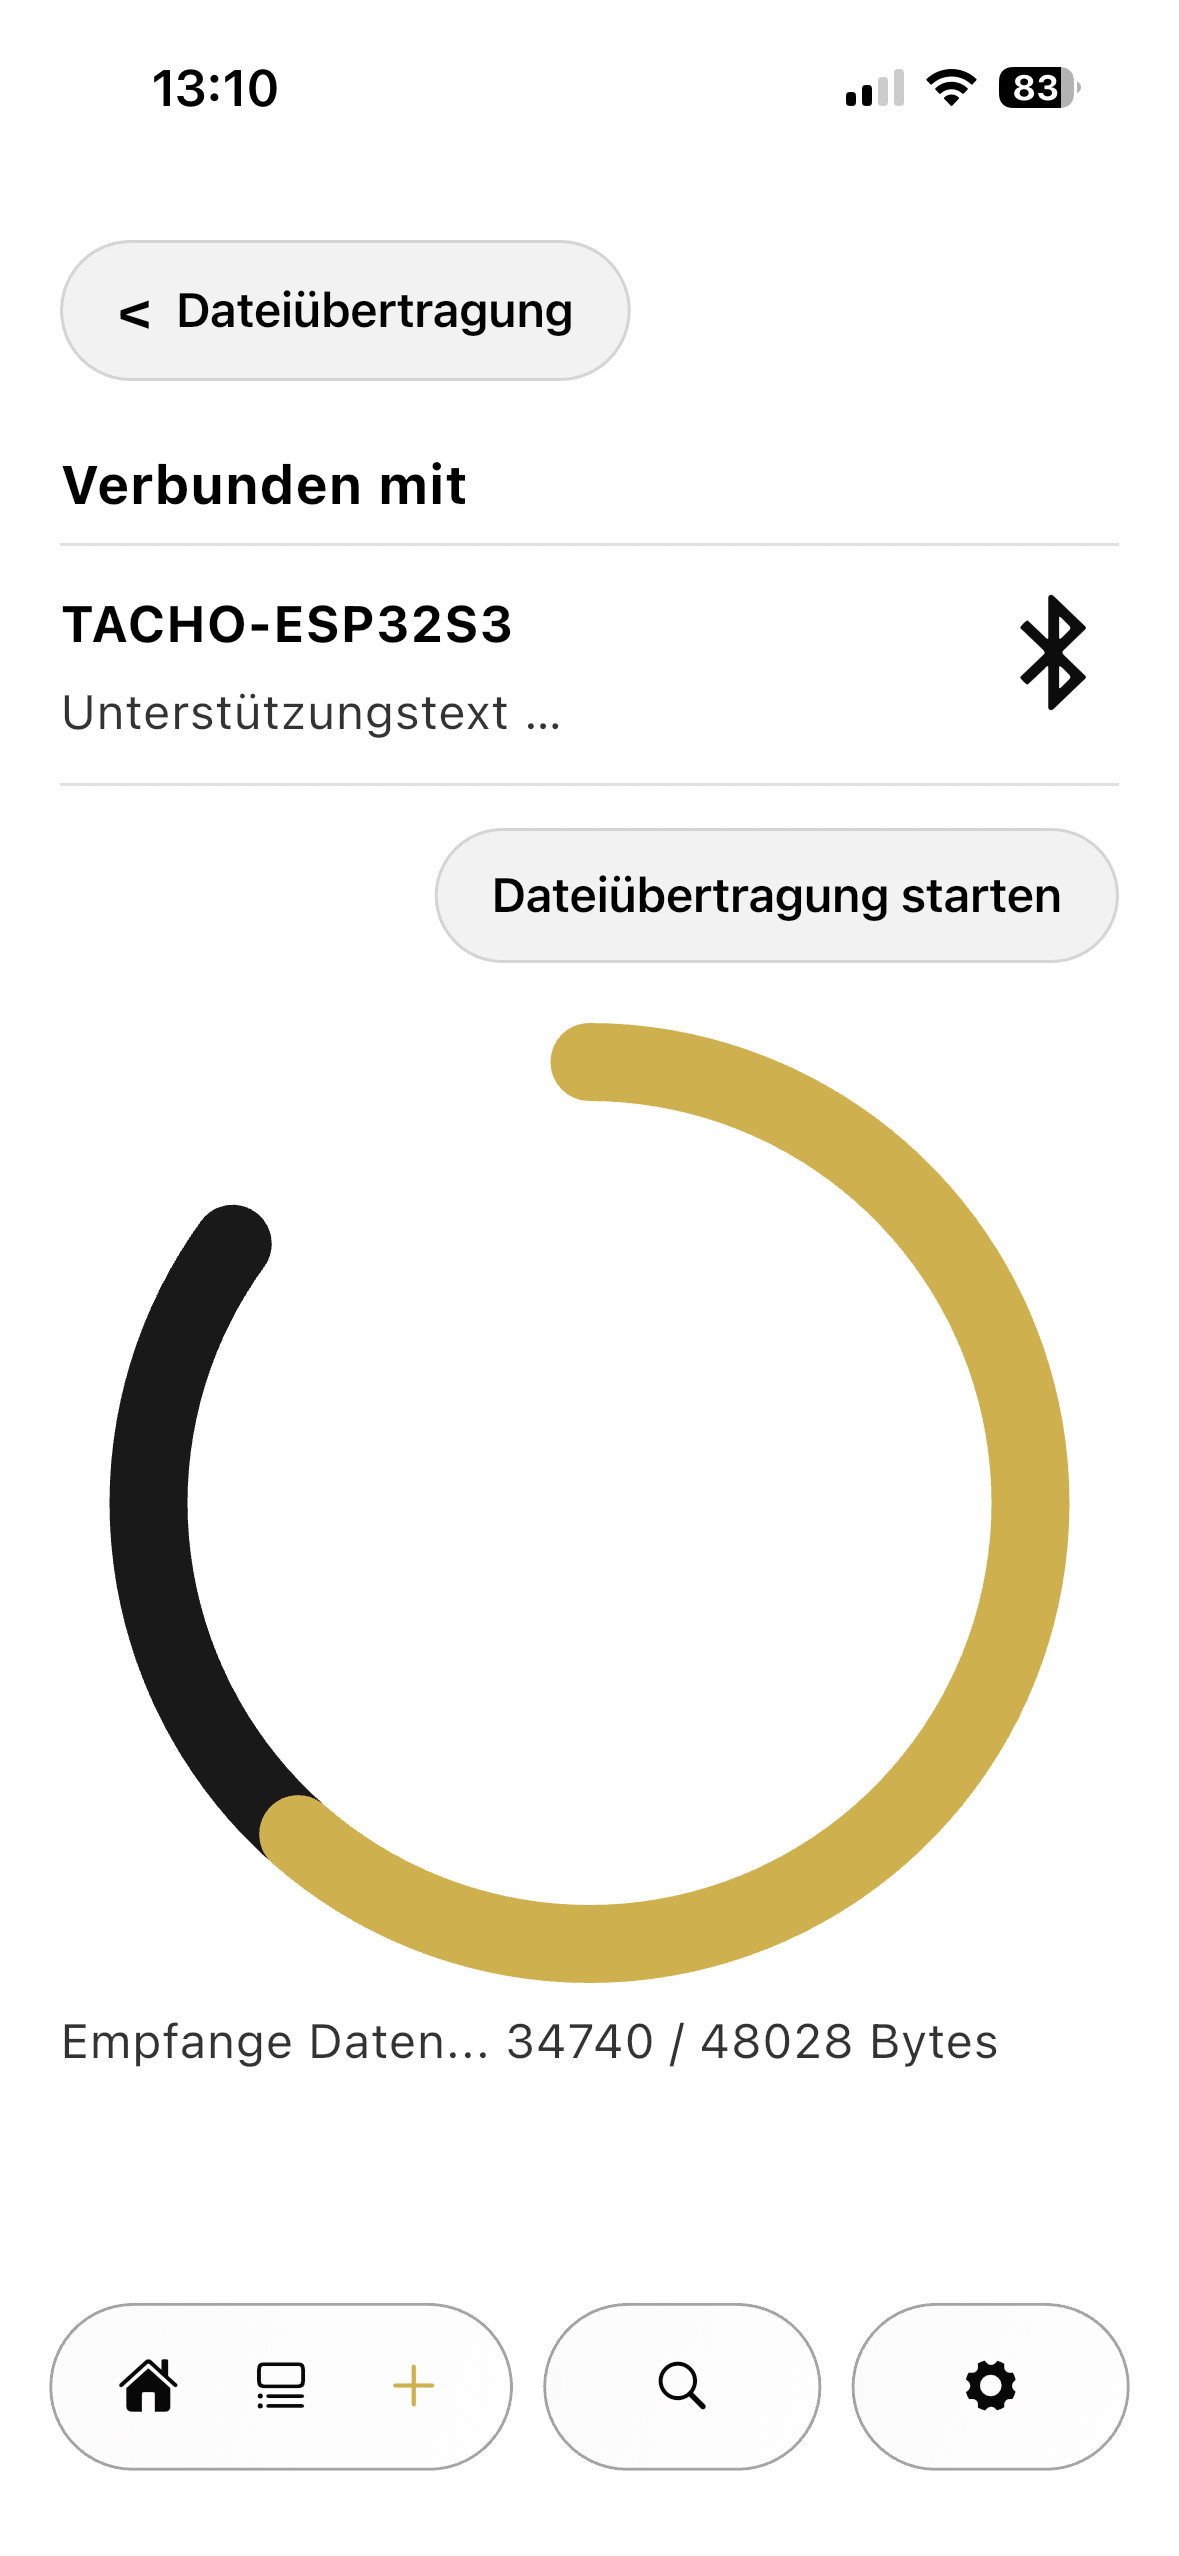
\includegraphics[width=\linewidth]{bilder/app8.png}
  \end{minipage}
  \caption{Verbindugsmenu und Dateiübertragung}
  \label{fig:app-ui-grid3}
\end{figure}
Das Verbindungsmenü bildet die Übertragung der Tachographendateien im \code{.ddd}-Format vom ESP32 über \gls{ble} ab. In der aktuellen Testumgebung übernimmt eine Demo-Software die Dateiübertragung, die eine BLE-Implementierung bereitstellt und eine \code{.ddd}-Datei aus dem Dateisystem übergibt. Nach dem Download werden die Daten geparst und strukturiert visualisiert. Zusätzlich zeigt die Anwendung technische Daten des Tachographen wie Hersteller, Seriennummer und Genehmigungsnummern sowie eine Downloadübersicht mit Kennzeichen des Fahrzeugs, Zeitpunkt des Downloads, aufgezeichnetem Zeitraum und Informationen zum letzten Download. Eine Systembenachrichtigung erinnert daran, sobald gesetzlich eine erneute Auslesung erforderlich ist.

\section{Geplante Erweiterungen}
Geplant sind ein Nutzerkonto mit Anbindung an eine Datenbank zur Zuordnung und zum Abruf von \code{.ddd}-Dateien sowie eine Suchfunktion für gezielte Abfragen. Zusätzlich soll das manuelle Hinzufügen von Tachographendateien ohne ESP32 möglich werden. Weitere Punkte sind Designanpassungen, eine integrierte Bedienungsanleitung und zusätzliche Hilfetexte.
